\documentclass[11pt]{utalcaDoc}
\usepackage{alltt}
\usepackage{underscore}
\usepackage[latin1]{inputenc}
\usepackage[activeacute,spanish]{babel}
\usepackage{verbatim}
\usepackage[pdftex]{graphicx}
\usepackage{ae}
\usepackage{amsmath}
\usepackage{amsfonts}
\usepackage{algorithm}
\usepackage{algorithmic}
\usepackage{float}
\floatname{algorithm}{Algoritmo}
\renewcommand{\listalgorithmname}{Lista de algoritmos}
\renewcommand{\algorithmicrequire}{\textbf{Precondici\'{o}n:}}
\renewcommand{\algorithmicensure}{\textbf{Postcondici\'{o}n:}}
\renewcommand{\algorithmicend}{\textbf{fin}}
\renewcommand{\algorithmicif}{\textbf{si}}
\renewcommand{\algorithmicthen}{\textbf{entonces}}
\renewcommand{\algorithmicelse}{\textbf{si no}}
\renewcommand{\algorithmicelsif}{\algorithmicelse,\ \algorithmicif}
\renewcommand{\algorithmicendif}{\algorithmicend\ \algorithmicif}
\renewcommand{\algorithmicfor}{\textbf{para}}
\renewcommand{\algorithmicforall}{\textbf{para todo}}
\renewcommand{\algorithmicdo}{\textbf{hacer}}
\renewcommand{\algorithmicendfor}{\algorithmicend\ \algorithmicfor}
\renewcommand{\algorithmicwhile}{\textbf{mientras}}
\renewcommand{\algorithmicendwhile}{\algorithmicend\ \algorithmicwhile}
\renewcommand{\algorithmicloop}{\textbf{repetir}}
\renewcommand{\algorithmicendloop}{\algorithmicend\ \algorithmicloop}
\renewcommand{\algorithmicrepeat}{\textbf{repetir}}
\renewcommand{\algorithmicuntil}{\textbf{hasta que}}
\renewcommand{\algorithmicprint}{\textbf{imprimir}} 
\renewcommand{\algorithmicreturn}{\textbf{devolver}} 
\renewcommand{\algorithmictrue}{\textbf{verdadero }} 
\renewcommand{\algorithmicfalse}{\textbf{falso }} 


\graphicspath{ {data/} }

\title{{\bf Dise�o de Software}\\Redesigning EDUCANDUS web application}
\author{Erik Regla\\ eregla09@alumnos.utalca.cl}
\date{\today}

\begin{document}
\renewcommand{\figurename}{Figura~}
\renewcommand{\tablename}{Tabla~}

\maketitle

\section{Overview of the document}
Universidad de Talca uses a Moodle platform to assist via e-learning their students and professors, but the current implementation is heavily patched to the core and lacks most of the desired features for their end users. In this report, we propose a new design to cover those problems detected by the author not considering details not relevant to the modifications design (such as login).

\section{Current issues detected by the community and our proposals to tackle them}

\subsection{Restricted communication between course participants}
Interaction between students and teachers is an important aspect of learning, but there is no way for students to communicate each other
by using this platform. Currently EDUCANDUS provides a forum system and email system which is synced with the alumni email and with 
course activities marked for notification.

Moreover, the forum system is readonly for students, hence they cannot communicate between themselves and the notification system 
tends to fail often. Also, there are times when the students need to work on their homework in groups (sometimes as large as the course
 itself), and the only way to communicate is to rely on SNSs like Facebook to do so. As the reader can expect, there is no way to provide 
 feedback in any direction for any of the available resources (namely assignments, course materials, etcetera) as now private messaging is disabled.
 
 
 
\subsubsection{Our proposal}
To solve this problem we need to design the following components:
\begin{enumerate}
\item \textbf{Direct messaging between course participants}
\item \textbf{General forum for the course}
\item \textbf{Resource forum}
\item \textbf{Group formation for assignments and private forum} %avoid realtime
\item \textbf{File upload capabilities for forums}
\end{enumerate}

\subsection{Lack of versioning of courses and resources}
There are two major points on both students and teachers argue against the current platform. Students always see former course 
contents, which leads to confusion when uploading homeworks and for students which are repeating the course, they get confused with 
their own submissions. 
On the other hand, teachers want to check former submissions and former course contents (by example, new teachers or when checking for plagiarism) and the platform erases it's content at the start of the semester. So they have to reupload all the content again and to deal
with repeated submissions.
When students upload their homeworks, there is no version control for the files that they are uploading to the platform, so, if the student makes an error by overwriting the correct file, there is no way to check if he is saying the truth.
\subsubsection{Our proposal}
To solve this problem we need to design the following components:
\begin{enumerate}
\item \textbf{Versioning at course level, including both contents and assignments}
\item \textbf{Versioning for the files uploaded to forums}
\end{enumerate}

\subsection{Grades not synced with the official grading platform (UTALMATICO)}
Class assistants and teachers often get confused about the grading system. The professor can communicate the grades that their students 
obtain in their assignments by uploading them on EDUCANDUS or UTALMATICO, but in the end only the latter counts to the grade registry 
used in the university. This means that grading homeworks on EDUCANDUS has no value and there can occur inconsistencies between 
the two platforms.

\subsubsection{Our proposal}
To solve this problem we need to design the following components:
\begin{enumerate}
\item \textbf{API consumer for EDUCANDUS platform, intended to be used with any grading system}
\item \textbf{Versioning for the files uploaded to forums}
\end{enumerate}



\subsection{Complex and useless assignment creation and management}
When creating assignments, there are tons of custom fields that aren't configured by default, like the grading scale used, deadline configuration and so on so forth. 
\subsubsection{Our proposal}
To solve this problem we need to design the following components:
\begin{enumerate}
\item \textbf{Standardised fields on assignments}
\end{enumerate}

We can summarise some of the most important use cases to be considered during the development stage in the following diagram.

\begin{figure}[H]
    \centering
	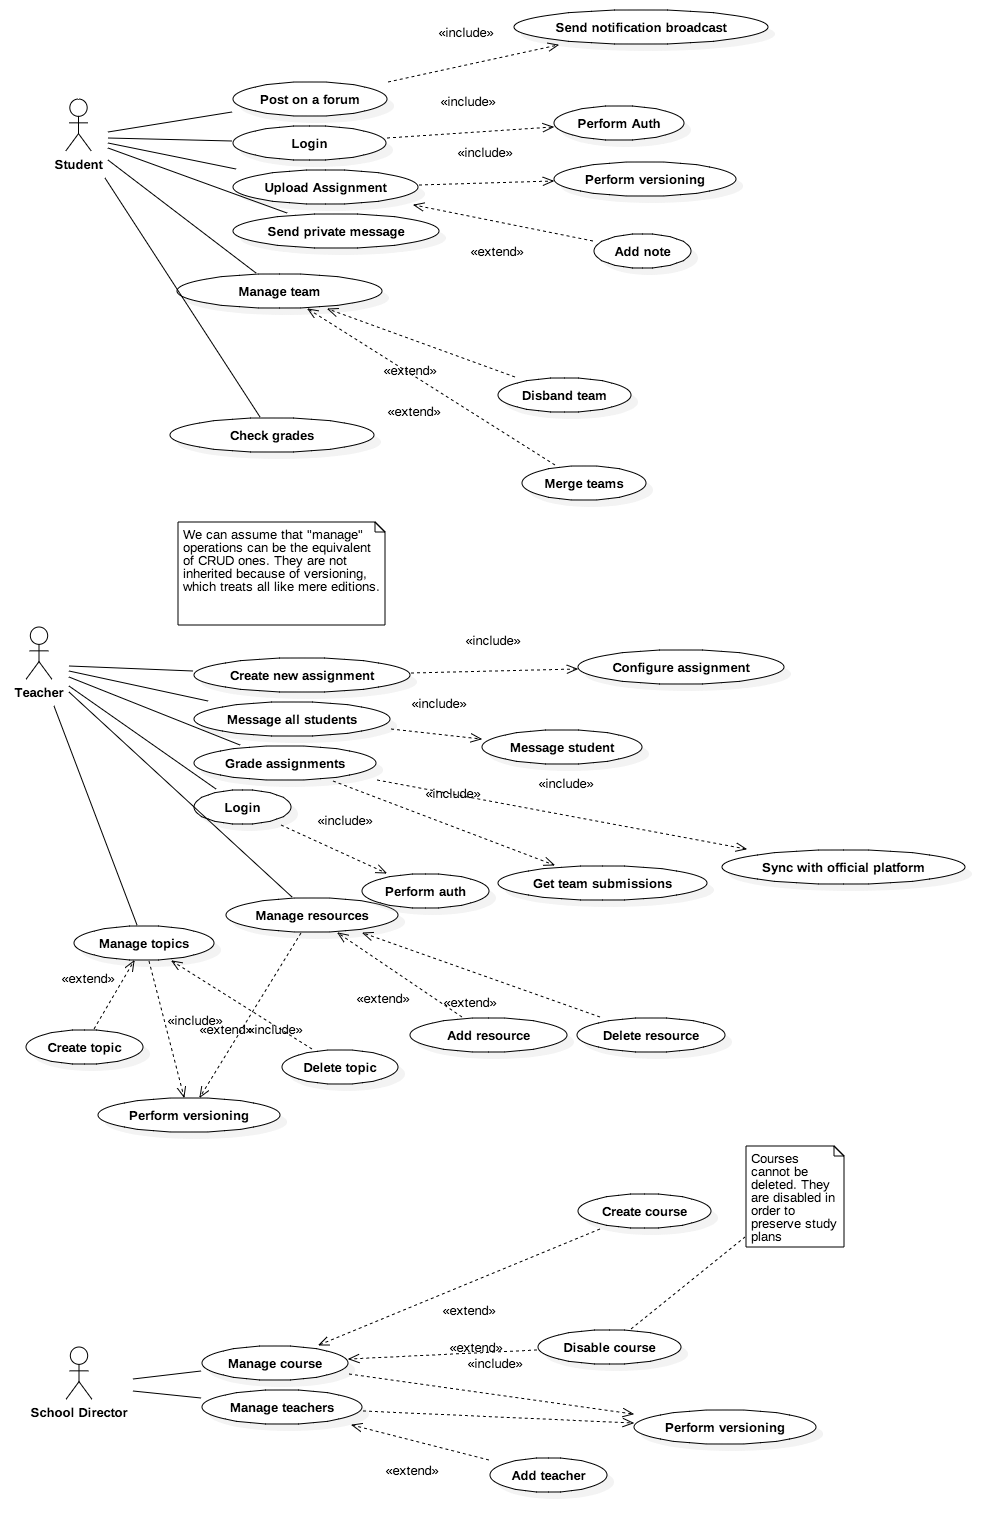
\includegraphics[width=\textwidth,height=\textheight,keepaspectratio]{UCD}
    \caption{Use case diagram for teachers, students and school directors}
    \label{UCD:GENERAL}
\end{figure}

\section{Domain Analysis}
Here we analyse the two most important domains in our design, the course and the forum. As seen, an improvement is the Ad-Hoc creation of teams. By default it is intended to create a team per person, then they can merge themselves to form a composed team. This enables us to implement team grading without changing our logic implementation.

Forums are pretty simple, just a collection of posts. We are aware that forums and realtime chat is already implemented on LMS but here we propose to enable them by default for each resource. This way we expect to motivate students to participate on rich discussions, open to all participants.

\begin{figure}[H]
    \centering
	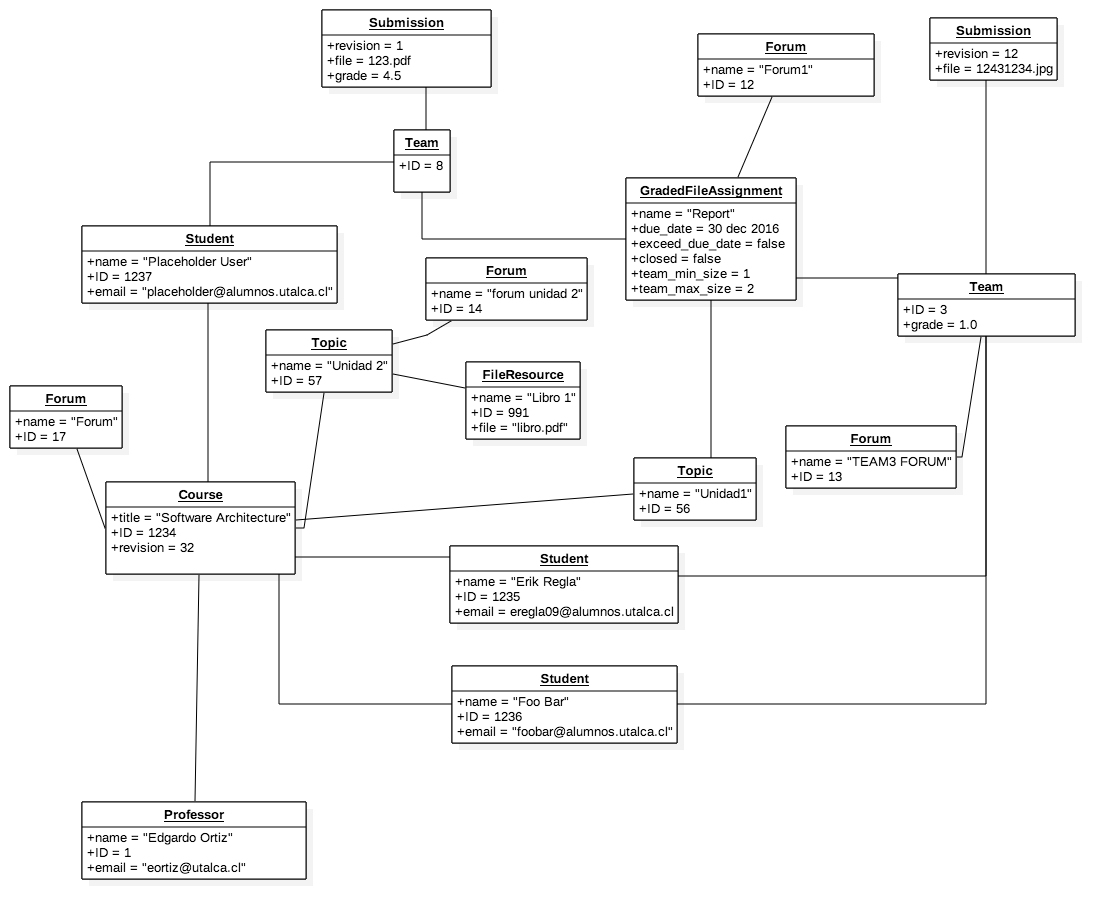
\includegraphics[width=\linewidth]{CourseTeamOD}
    \caption{Object diagram for course, students, resources, assignments and teams}
    \label{OD:COURSE_TEAM}
\end{figure}

\begin{figure}[H]
    \centering
	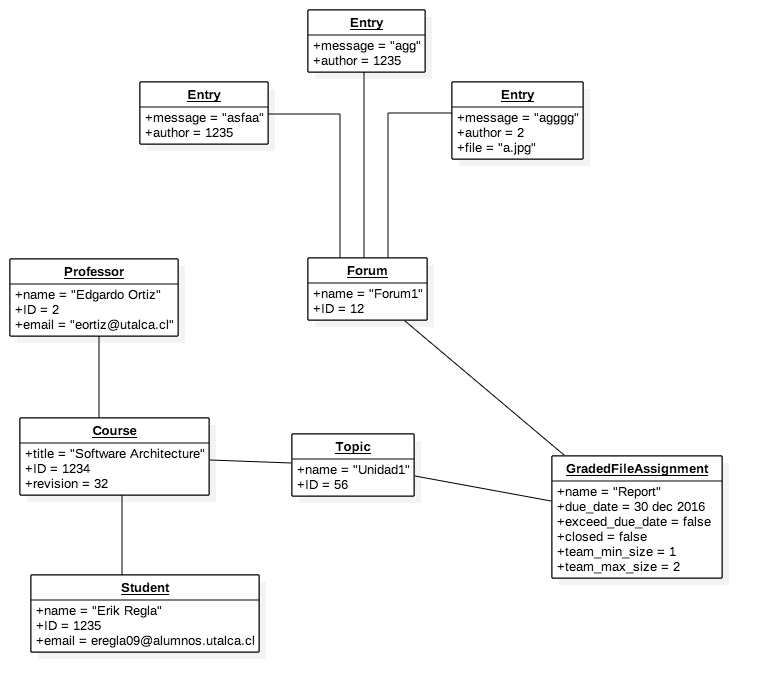
\includegraphics[width=\linewidth]{ForumOD}
    \caption{Object diagram for forums and participants}
    \label{OD:COURSE_TEAM}
\end{figure}

Other diagrams like login, plugins, etcetera are not included as they do not improve the understanding of the problem.
%%OD diagrams
\subsection{Users}
Users are restricted to three types: School directors, Teachers and Students. At module level, they do not have any extra information, because the login module is in charge to administer all the permisions involved. This is necessary because some students are actually class assistants and they need permissions to edit course materials. When this happens, a petition must be elevated using the management system which is covered in detail later.

\begin{figure}[H]
    \centering
	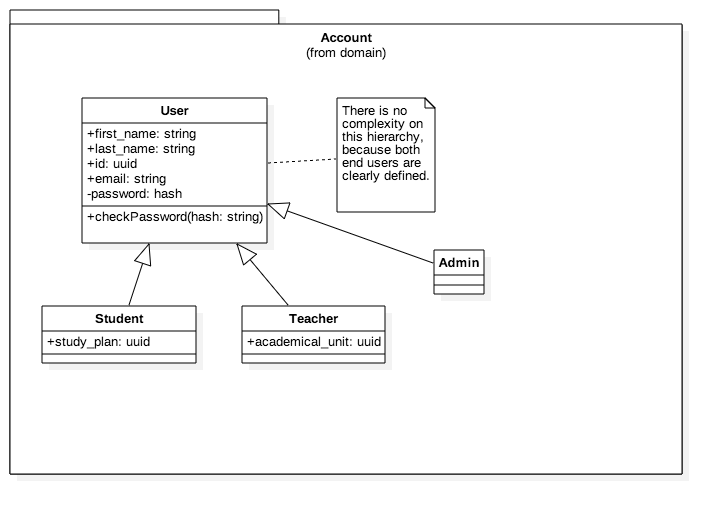
\includegraphics[width=\linewidth]{UsersCD}
    \caption{Users package}
    \label{CD:USERS}
\end{figure}


\subsection{Forums}
Forums can be seen in two ways, at a resource/conversation level or as a course. We already stated that every resource should have a forum to help public communication and opinion sharing in realtime. By realtime we do not mean to implement a chat system, since it can encourage students to not think before they write and to discuss complex topics that will require images and media can be troublesome.

Forums should reveal a composite design, because we can think a course as a tree of resources more than a list of them, therefore, if one desires to access a course forum, all topics and threads should be seen in the same hierarchy as the course has. Then, aside from the typical implementation of the forum structure, we need an adapter to export the forums to the versioning system and back on. This can be achieved by implementing any serialisation interface as long as the interface remains the same.

\begin{figure}[H]
    \centering
	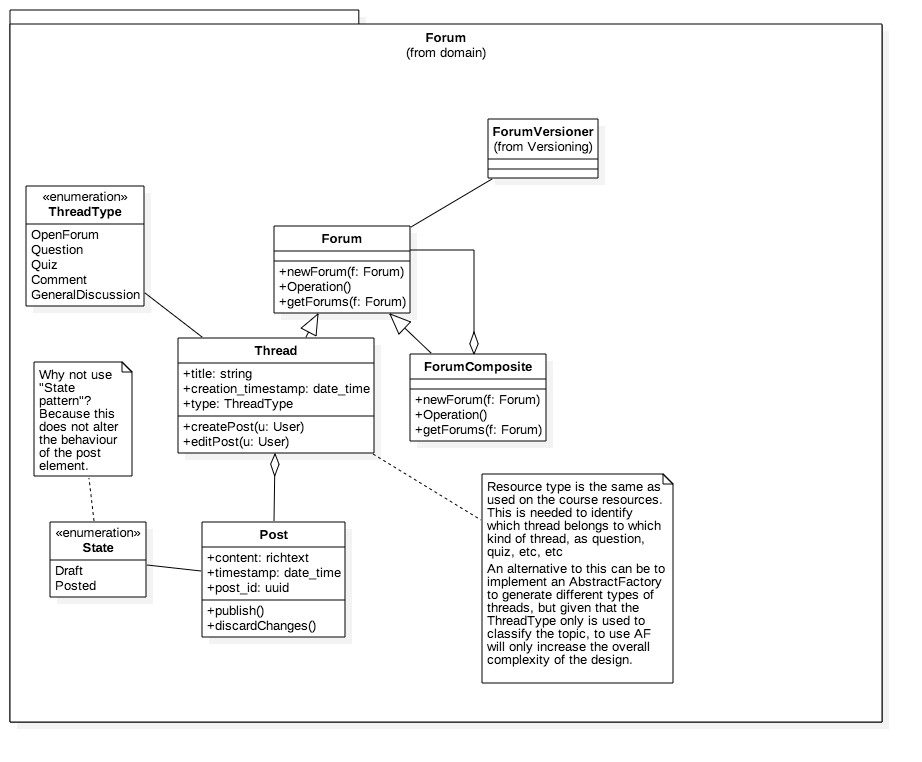
\includegraphics[width=\linewidth]{ForumCD}
    \caption{Forum package}
    \label{CD:FORUM}
\end{figure}

\subsection{Versioning}
Versioning is supposed to operate in a different level than forums and users, much alike an adapter or a bridge to another versioning system (which could be SVN, GIT, etc), wihout exposing how versioning should be performed but giving a standard set of operations to version each element of the platform.

The mechamism is much like the same for every element present, the resource is serialised, then passed as a memento to the versioning system. The platform sees each version as a memento, whilst the versioning system is ready to pass this serialised (or maybe not) data onto the underlying versioning platform.

\begin{figure}[H]
    \centering
	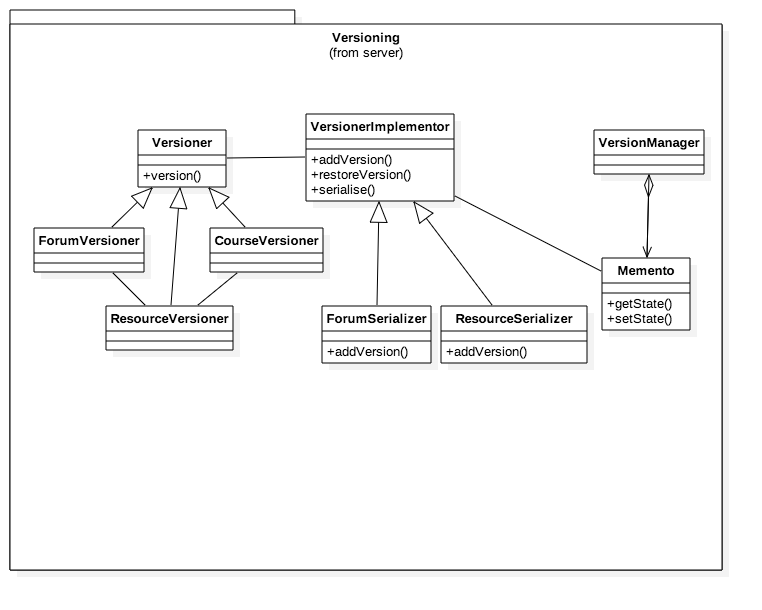
\includegraphics[width=\linewidth]{VersioningCD}
    \caption{Versioning package}
    \label{CD:VERSIONING}
\end{figure}

\begin{figure}[H]
    \centering
	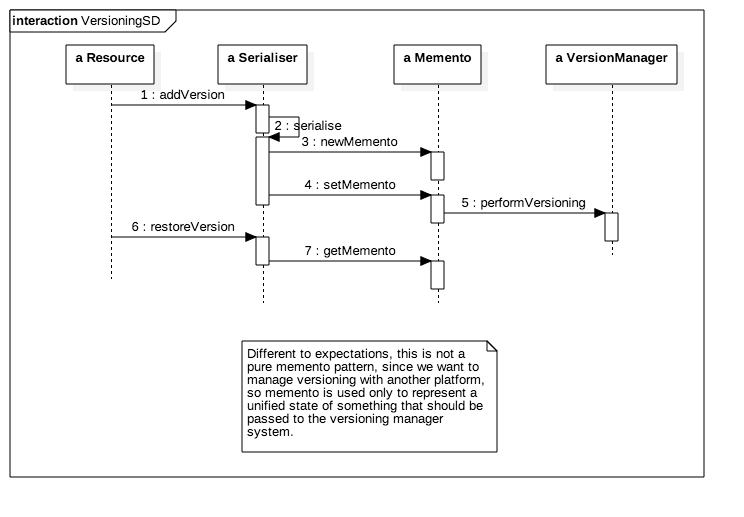
\includegraphics[width=\linewidth]{VersioningSD}
    \caption{Versioning interactions}
    \label{SD:VERSIONING}
\end{figure}



\section{Domain Design and High Level Domain Analysis}
\begin{figure}[H]
    \centering
	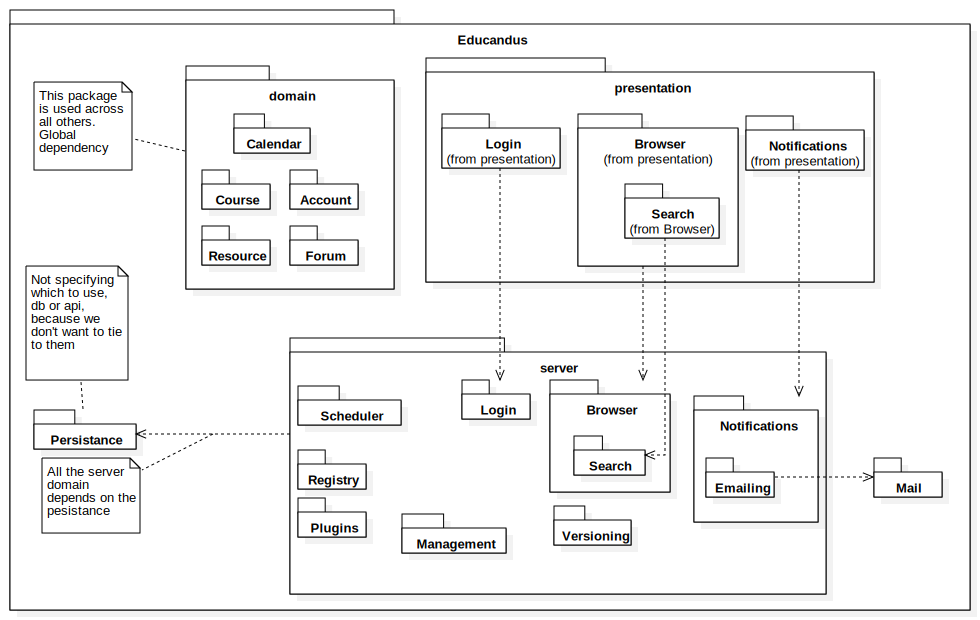
\includegraphics[width=\linewidth]{PackageArchitecture}
    \caption{Package architecture of the application}
    \label{PD:ARCHITECTURE}
\end{figure}



We can think of this application as a simple producer-consumer model for the end users, moreover, there are some processes that need to pay close attention. Whilst the view only consumes and triggers commands on the server, the server itself needs to perform several operations by its own. Therefore, we choose to implement a multi-layered architecture on where the main modules are:
\begin{enumerate}
\item Presentation layer
\item Serverside layer
\item Mailing
\item The official grading platform API
\end{enumerate}

\section{Package and Implementation Architecture}


\end{document}